
% xetex expected
\documentclass[xetex,professionalfont]{beamer}

% we want math
\usepackage{amsmath}

% fixes and extensions to amsmath
\usepackage{mathtools}

% additional math symbols
\usepackage{amssymb}

% good-looking fractions in text via \sfrac
\usepackage{xfrac}

% fix spaces after custom commands (see below for examples)
\usepackage{xspace}

% minted allows for fancy syntax highlighting (requires python with pygments)
% usage:
%   \begin{minted}{python}
%   codeb
%   \end{minted}
% \usepackage{minted}

% better looking tables
% usage:
%   begin with a \toprule, write a single row of column headings,
%   then add \midrule and after the columns of data we finish with \bottomrule
% example:
%   \begin{tabular}{llr} \toprule
%   Animal & Description & Price \midrule
%   cat & foo & 10 \\
%   dog & bar & 20 \\ \bottomrule
%   \end{tabular}
% note that good tables generally neither have vertical rules nor double rules
\usepackage{booktabs}

% system font support (requires xetex or luatex)
\usepackage{fontspec}
\setmonofont[Scale=0.7]{Cousine} % part of ttf-chromeos fonts on Arch

% improve microtypography
\usepackage{microtype}

% multi-language quotes for babel
\usepackage{csquotes}

% easy way to include copyright information
\usepackage{copyrightbox}

% better bibliographies
\usepackage[backend=biber,style=authoryear]{biblatex}

% language support (english,ngerman)
\usepackage[english]{babel}

% -----------------------------------------------------------------------------

% specify PDF metadata
\hypersetup{pdftitle={CVSP UE - Preview},pdfsubject={},pdfauthor={Christopher Pramerdorfer}}

% copyright font style
\makeatletter\renewcommand{\CRB@setcopyrightfont}{\tiny\color{lightgray}}

% make emph bold
\DeclareTextFontCommand{\emph}{\bfseries}

% use tuwcvl beamer theme
\usetheme{tuwcvl}

% -----------------------------------------------------------------------------

% common english abbreviations
\newcommand{\ie}{\mbox{i.e.}\xspace} % i.e.
\newcommand{\eg}{\mbox{e.g.}\xspace} % e.g.

% math - argmin and argmax
\DeclareMathOperator*{\argmin}{arg\,min}
\DeclareMathOperator*{\argmax}{arg\,max}

% shortcuts for number ranges
\newcommand{\NN}{\mathbb{N}}
\newcommand{\ZZ}{\mathbb{Z}}
\newcommand{\QQ}{\mathbb{Q}}
\newcommand{\RR}{\mathbb{R}}

% bold vectors
\renewcommand{\vec}[1]{\ensuremath{\mathbf{#1}}}

% vector shortcuts
\newcommand{\va}{\vec{a}}
\newcommand{\vb}{\vec{b}}
\newcommand{\vc}{\vec{c}}
\newcommand{\ve}{\vec{e}}
\newcommand{\vr}{\vec{r}}
\newcommand{\vs}{\vec{s}}
\newcommand{\vt}{\vec{t}}
\newcommand{\vu}{\vec{u}}
\newcommand{\vv}{\vec{v}}
\newcommand{\vw}{\vec{w}}
\newcommand{\vx}{\vec{x}}
\newcommand{\vy}{\vec{y}}
\newcommand{\vz}{\vec{z}}

% -----------------------------------------------------------------------------

\title{Computer Vision Systems Programming UE}
\subtitle{Introduction}
\author{Christopher Pramerdorfer}
\institute{Computer Vision Lab, Vienna University of Technology}

\begin{document}

% -----------------------------------------------------------------------------

\begin{frame}
\maketitle
\end{frame}

% -----------------------------------------------------------------------------

\begin{frame}
\frametitle{Course Topics}

Motivation
\begin{itemize}
	\item Computer Vision (CV) knowledge is important
	\item As is to be able to \emph{put this knowledge to use}
\end{itemize}

\bigskip
This course encourages you to
\begin{itemize}
	\item Explore a CV topic of your choice
	\item Get used to software packages and libraries
	\item Improve your CV programming skills
\end{itemize}

\end{frame}

% -----------------------------------------------------------------------------

\begin{frame}
\frametitle{Your Task}

Select, implement, and present a CV project of your choice
\begin{itemize}
	\item In any programming language you like
	\item Using any \emph{publicly available} libraries you want
	\item As long as the required effort is appropriate
\end{itemize}

\bigskip
Matlab, Python, or C++ recommended

\end{frame}

% -----------------------------------------------------------------------------

\begin{frame}
\frametitle{Project Topics}

Choose any CV topic you want, as long as you learn something
\begin{itemize}
	\item Choose something that is new and interesting to you
	\item Finalize topic and scope in consultation with lecturers
\end{itemize}

\bigskip
Don't know what topic to choose? How about these ...

\end{frame}

% -----------------------------------------------------------------------------

\begin{frame}
\frametitle{Project Topics}
\framesubtitle{Proposal -- Balloon Tracking}

Involve concert audience by letting them control sound aspects\\\medskip
Accomplished by moving a balloon above their heads

\bigskip
\begin{center}
	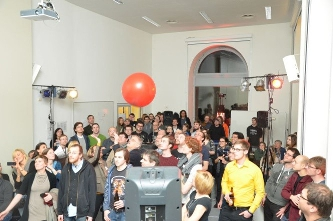
\includegraphics[width=6cm]{figures/balloon.jpg}
\end{center}

\end{frame}

% -----------------------------------------------------------------------------

\begin{frame}
\frametitle{Project Topics}
\framesubtitle{Proposal -- Balloon Tracking}

Task: detect and track the balloon in 3D
\begin{itemize}
	\item Camera parameters and balloon size are known
	\item Pose estimation problem
\end{itemize}

\bigskip
Extensions
\begin{itemize}
	\item Detect balloon color
	\item Track multiple balloons simultaneously
\end{itemize}

\medskip
\begin{center}
	\small\url{http://www.caa.tuwien.ac.at/cvl/teaching/praktika/ballonerkennung/}
\end{center}

\end{frame}

% -----------------------------------------------------------------------------

\begin{frame}
\frametitle{Project Topics}
\framesubtitle{Proposal -- Meal Composition Recognition}

Unhealthy nutrition is a problem in our society\\\medskip
Often there is little knowledge of the composition of meals

\bigskip
\begin{center}
	\copyrightbox[b]
	{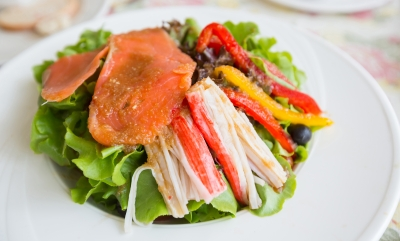
\includegraphics[width=6cm]{figures/meal.jpg}}
	{\centering Image by Vichaya Kiatying-Angsulee / \url{freedigitalphotos.net}}
\end{center}

\end{frame}

% -----------------------------------------------------------------------------

\begin{frame}
\frametitle{Project Topics}
\framesubtitle{Proposal -- Meal Composition Recognition}

Task: estimate share of carbs, proteins, vegetables in meals\\\medskip
From photos taken with smartphone cameras

\medskip
\begin{center}
	\small\url{http://www.caa.tuwien.ac.at/cvl/teaching/praktika/food/}
\end{center}

\end{frame}

% -----------------------------------------------------------------------------

\begin{frame}
\frametitle{Project Topics}
\framesubtitle{Proposal -- Sitting Posture Recognition}

Bad sitting posture can cause health problems\\\medskip
Task: recognize good or bad posture using a Kinect sensor

\bigskip
\begin{center}
	\copyrightbox[b]
	{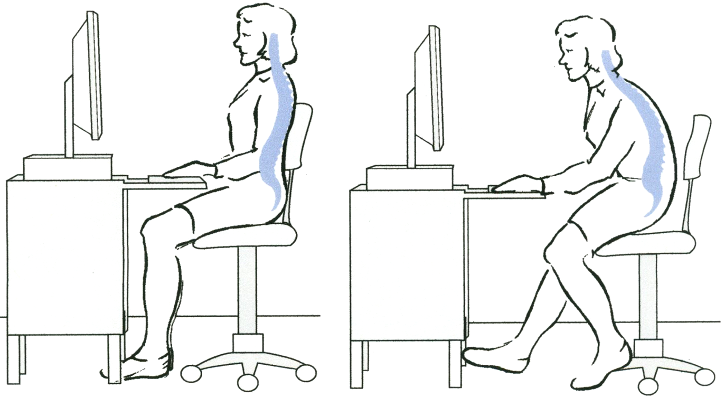
\includegraphics[width=6cm]{figures/sitting.png}}
	{\centering Image from \url{yogahome.net}}
\end{center}

\end{frame}

% -----------------------------------------------------------------------------

\begin{frame}
\frametitle{Project Topics}
\framesubtitle{Proposal -- Kinect v2 Evaluation}

Evaluate the Kinect v2 sensor

\bigskip
\begin{center}
	\copyrightbox[b]
	{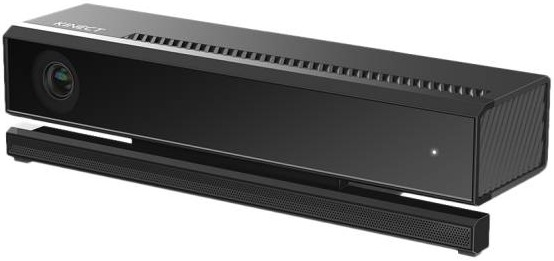
\includegraphics[width=6cm]{figures/kinect.jpg}}
	{\centering Image from \url{microsoftstore.com}}
\end{center}

\end{frame}

% -----------------------------------------------------------------------------

\begin{frame}
\frametitle{Project Topics}

Send a short project proposal to lecturers (\url{cvsp@caa.tuwien.ac.at})
\begin{itemize}
	\item What topic do you want to cover
	\item What is the scope (what are you going to implement?)
	\item What language and libraries do you plan to use
\end{itemize}

\bigskip
Do so as soon as possible (\emph{deadline: 26.10.})

\end{frame}

% -----------------------------------------------------------------------------

\begin{frame}
\frametitle{Syllabus}

1.\ Select a CV topic according to your interests
\begin{itemize}
	\item Lecturers will help you define topic and scope
\end{itemize}

\medskip
2.\ Give a short presentation on your topic (5 minutes)
\begin{itemize}
	\item Explain what you are going to work on
\end{itemize}

\medskip
3.\ Implement and test your application
\begin{itemize}
	\item Sensor hardware is provided
\end{itemize}

\medskip
4.\ Write a short report (around 5 pages)

\medskip
5.\ Give a final presentation (10-15 minutes)

\end{frame}

% -----------------------------------------------------------------------------

\begin{frame}
\frametitle{Syllabus}
\framesubtitle{Available Sensor Hardware}

Available sensors
\begin{itemize}
	\item Kinect depth sensors
	\item IP camera network with overlapping views (stationary)
	\item Thermal imaging camera (stationary)
	\item Android tablets with cameras
\end{itemize}

\bigskip
Or use your own digital camera, smartphone, ...

\end{frame}

% -----------------------------------------------------------------------------

\begin{frame}
\frametitle{Syllabus}
\framesubtitle{Short report and Final Presentation}

Report and presentation should include
\begin{itemize} 
	\item A brief explanation of your topic
	\item How you implemented it (language, libraries)
	\item Problems you faced during development
	\item Tests and results
\end{itemize}

\end{frame}

% -----------------------------------------------------------------------------

\begin{frame}
\frametitle{Course Location and Schedule}

There are no regular lectures but two presentation meetings

\bigskip
\textbf{Location}: Seminarraum 183/2, Favoritenstr. 9\\
\textbf{Time}: Wed 10:15 -- 11:45 s.t.

\bigskip
\textbf{Schedule}: \url{http://www.caa.tuwien.ac.at/cvl/teaching/wintersemester/cvsp_lu/index.html}

\bigskip
Follow \texttt{@tuwcvsp} on Twitter for updates

\end{frame}

% -----------------------------------------------------------------------------

\begin{frame}
\frametitle{Course Assistance}

Assistance mainly via mail (\url{cvsp@caa.tuwien.ac.at})

\bigskip
Weekly timeslot for personal support
\begin{itemize}
	\item \textbf{By appointment} (\url{cvsp@caa.tuwien.ac.at})
	\item \textbf{Time}: Wed 11:45 -- 12:30 s.t. (after VO)
	\item \textbf{Location}: room HA04-10 \scriptsize\url{http://www.caa.tuwien.ac.at/cvl/contact/floorplan.html}\normalsize
\end{itemize}

\bigskip
We expect to stay in touch with you throughout the semester

\end{frame}

% -----------------------------------------------------------------------------

\begin{frame}
\frametitle{Course Assistance}

I'm abroad from 11.10.\ to 25.10.\ with limited internet access

\end{frame}

% -----------------------------------------------------------------------------

\begin{frame}
\frametitle{Prerequisites}

You must be able to develop software on your own
\begin{itemize}
	\item This is \emph{not} a general programming course
\end{itemize}

\bigskip
Basic image processing and computer vision knowledge

\end{frame}

% -----------------------------------------------------------------------------

\begin{frame}
\frametitle{Grading}

Initial presentation: 5\% \\
Implementation and report: 80\% \\
Final presentation: 15\%

\bigskip
\emph{Presentations are mandatory!}

\end{frame}

% -----------------------------------------------------------------------------

\begin{frame}
\frametitle{Associated Lecture}

We recommend the associated lecture that covers
\begin{itemize}
	\item CV software and resources
	\item Selected CV applications
\end{itemize}

\end{frame}

\end{document}